\chapter{CIDR Report characteristics \& influence on AS behavior}
\label{chap:analysis}

This chapter presents and describes observed characteristics of the CIDR
Report, as well as the results of the analysis conducted to determine if the
CIDR Report affects network operator route aggregation behavior. The chapter
begins with a preliminary discussion about the availability of data and the
quality of our aggregation report implementation. This is followed by
presentation of characteristics of the CIDR report that were observed during
this analysis, which will be discussed in the following chapter as clues of
what may have affected the success of the CIDR Report. The chapter continues
with presentation of the main results of the analysis relevant to this thesis,
illustrating how individual ASes' route announcement behavior may have been
affected by appearing on the CIDR Report. Finally, potential questions about
the validity of the analysis are identified and discussed.

As discussed briefly in the previous chapter, there are two data sets at play
in this analysis. The distinction between these two sets is important for
understanding some of the figures in this section, and so they are clearly
defined here:

\begin{itemize}

\item{The authoritative CIDR Report (ACR): This is the data from the
authoritative CIDR Report that was emailed out to network operators that
identifies the 30 most deaggregated ASes.  This is the set of ASes that would
be expected to display a treatment effect if the CIDR Report was effective.}

\item{The generated CIDR Report (GCR): This is the full aggregation report
generated by our implementation of the prefix aggregation algorithm used by the
CIDR Report, but containing data for every AS in the routing table instead of
being truncated after the 30th AS.}

\end{itemize}

Finally, to refresh the reader, some terms of art will be used in the remainder
of the chapter for conciseness. These are:

\begin{itemize}

\item{\emph{netgain:} The number of prefixes advertised by an AS that are
unnecessary (do not affect routing policy from the perspective of the CIDR
Report vantage point), and could be removed from the routing table if this AS
aggregated perfectly.}

\item{\emph{netsnow:} The total number of prefixes advertised by an AS,
including both aggregable and non-aggregable routes.}

\end{itemize}

\section{Data and methodological quality}

\subsection{Data availability}

The historic origins and other peculiarities of the underlying data sources for
the ACR and GCR mean that the data series for two reports start at different
dates and contain small gaps in their otherwise continuous record of weekly
CIDR Report data. The start dates and gaps are illustrated in Figure
\ref{fig:avail_data}, where a solid vertical line indicates a week of available
data.

\begin{figure}[h!]
\begin{centering}
\begin{singlespace}
    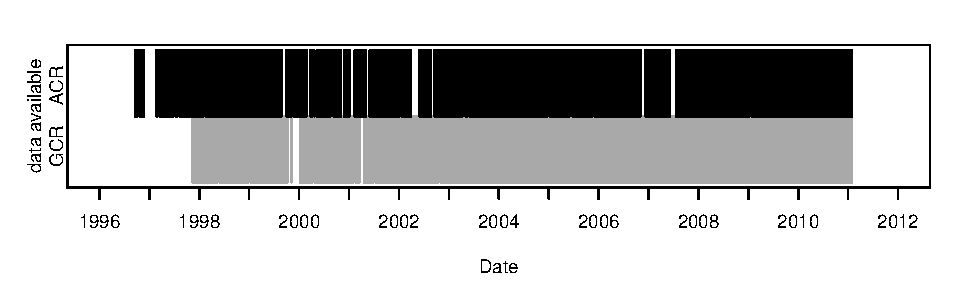
\includegraphics[width=6in]{figures/data_avail.pdf}
    \vspace{-2em}\\
    \caption{Available data}
    \label{fig:avail_data}
\end{singlespace}
\end{centering}
\end{figure}

As illustrated, data from both reports is generally available from November 1997
until January 2011, with a few relatively minor gaps. The period where the ACR
and GCR data overlap is the period used to analyze the effects of the CIDR
Report on AS behavior.

%	- plot total prefixes in the total table (Routeviews) and in the report (CIDR Report) to see that there aren't any discontinuities
% this is the "peer count" that I allude to

\subsection{GCR implementation accuracy}

In addition to data availability, the accuracy of the analysis that follows also
depends on the accuracy of our implementation of the CIDR Report aggregation
algorithm described in Chapter \ref{chap:method}. Recall that while the ACR is
used to determine when an AS appears on the CIDR Report (and thus potentially
commands attention of the community), the GCR is used to determine actual
post-appearance behavior because it provides consistently-generated measures
(like the number of aggregable prefixes advertised, \emph{netgain}) for ASes
both above and below the ACR top 30 threshold.

The first measure of accuracy is a comparison of the aggregable and total
prefixes determined for each AS on the ACR and GCR. A plot illustrating this
comparison is shown in Figure \ref{fig:comp_prefix_error}. The curves above the
horizontal zero ($y=0$) represent the sum of the differences in prefix counts
between the ACR and GCR for ASes where the GCR reports more prefixes than the
ACR. Similarly, the curves below the zero represent the sum of differences in
prefix counts between the ACR and GCR for ASes where the ACR reports more
prefixes than the GCR. The total deviation between the ACR and GCR is
given by the difference between the curves above and below zero.

\begin{figure}[h!]
\begin{centering}
\begin{singlespace}
    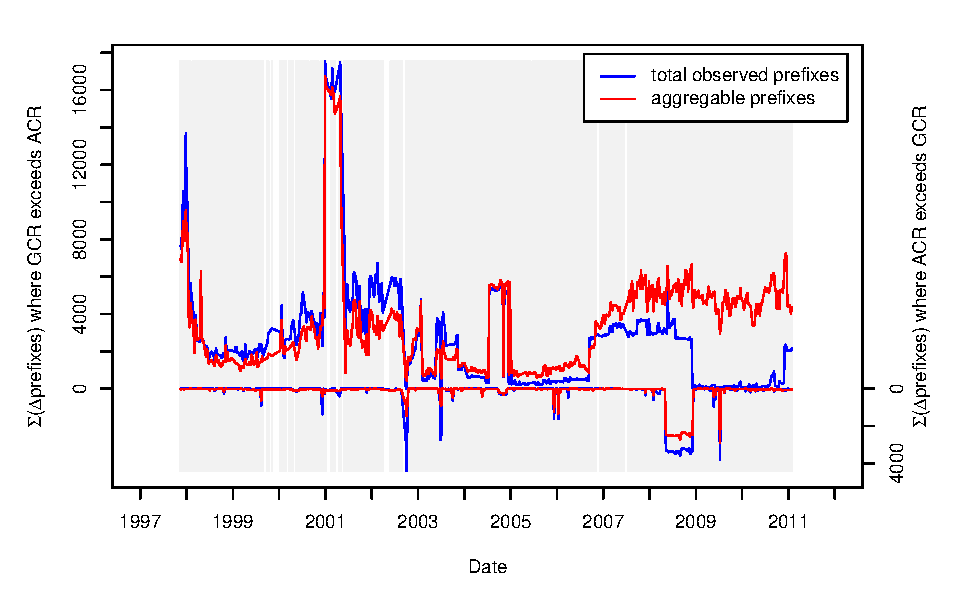
\includegraphics[width=6in]{figures/cidr_report_validity_prefix_error.pdf}
    \vspace{-2em}\\
    \caption{Differences in prefix counts between authoritative (ACR) and
        generated (GCR) CIDR Reports over time.}
    \label{fig:comp_prefix_error}
\end{singlespace}
\end{centering}
\end{figure}

As can be seen in Figure \ref{fig:comp_prefix_error}, throughout the period of
available data, the GCR generally claims larger quantities of aggregable and
total prefixes than the ACR. This is particularly pronounced and erratic when
compared against the pre-August 2002 CIDR Report (the point when the report's
methodology was changed when it was re-implemented by Geoff Huston). It is
difficult to determine the cause of this, but we suspect it is due to the
greater number of vantage points used in generating the GCR, leaving the GCR
more open to observing prefixes not visible from the ACR vantage point or
observing AS\_PATHs that enable classification of prefixes as aggregable.

After August 2002, agreement between the ACR and GCR improves, though there are
still inconsistencies. Most of these inconsistencies appear attributable to
the GCR observing more prefixes than the ACR---this is the case when the
observed prefixes (blue line) and aggregable prefixes (red line) increase
simultaneously. Perhaps more concerning in terms of accuracy is the change in
behavior that began in late 2008 and continues to the latest, where the ACR and
GCR observe the same number of prefixes (blue line is approximately zero) but
the GCR classifies 4000-5000 more prefixes as aggregable. Upon further
investigation, these deviations appeared to be due to the multiple vantage
points used by the GCR, which observed potential aggregation that the ACR did
not observe.

In spite of these inconsistencies, which are generally minor in terms of
ACR-GCR disparity for individual ASes, the GCR presents a view of potential
routing table aggregability that is sufficiently consistent with the ACR to
enable our use of the GCR as a data source for analyzing individual AS
aggregation behavior after appearing on the CIDR Report. Further, because data
related to prefix counts is always taken from the GCR, prefix data and
differences calculated based on this data will always be consistent and not
affected by differences between the ACR and GCR. Finally, as will be discussed
next, these minor differences in prefix counts do not greatly affect the ranks
of ASes on the GCR when compared to the ACR.

While it is helpful to look at differences in prefix counts, as this is the
major purpose for which the GCR is used (rather than the ranking it generates),
we can also compare the rankings it generates against the rankings from the ACR
to compare the relative accuracy of the GCR. Ranks provided by the GCR are not
currently used in this analysis, so we only briefly raise this before continuing
on.

Figure \ref{fig:comp_rank_error} illustrates the minimum and maximum absolute
differences between the ranks of ASes appearing on the ACR and the ranks of
corresponding ASes on the GCR.

\begin{figure}[h!]
\begin{centering}
\begin{singlespace}
    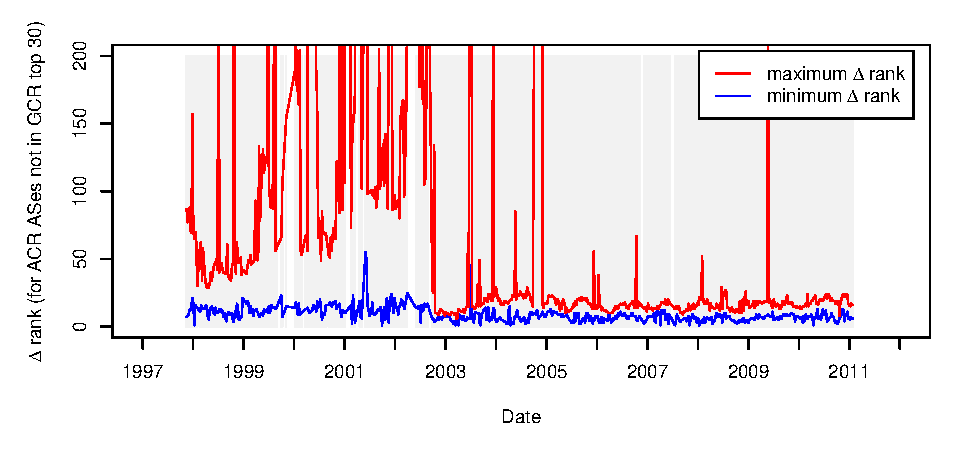
\includegraphics[width=6in]{figures/cidr_report_validity_rank_error.pdf}
    \vspace{-2em}\\
    \caption[Minimum and maximum differences in aggregation report
    rank]{Minimum and maximum differences in aggregation report rank for ASes
    ranked in the top 30 on the ACR but not in the top 30 on the GCR.}
    \label{fig:comp_rank_error}
\end{singlespace}
\end{centering}
\end{figure}

As can be seen, similar to the differences in prefix counts shown in the
previous figure, the rank differences are more significant and erratic from
1997 until August 2002, at which point they become more consistent. With some
exceptions, likely due to input data aberrations, the rankings generally differ
only a small amount, often near zero in the best case and no more than 20-30
in the worst case. Also, typically 20-25 of the ASes that appear on the ACR
also appear on the GCR.

% While not captured in the above plot, the differences between rankings on the
% ACR and GCR are generally at the top of the report and are generally a result
% of the GCR observing more potential aggregation than the ACR did, resulting in
% a different set of ASes at the top of the GCR than at the top of the ACR. The
% ASes at the top of the ACR thus typically rank lower on the GCR, because they
% have lower netgain than the most deaggregated ASes observed by the GCR. This
% means that in spite of the large rank differences displayed,

% Figure \ref{fig:comp_top30_error} illustrates the total number of ASes ranked
% in the top 30 of the ACR that are not also in the top 30 of the GCR, as well as
% the rank of the first AS on the ACR not in the top 30 of the GCR.
%
% \begin{figure}[H]
% \begin{centering}
% \begin{singlespace}
%     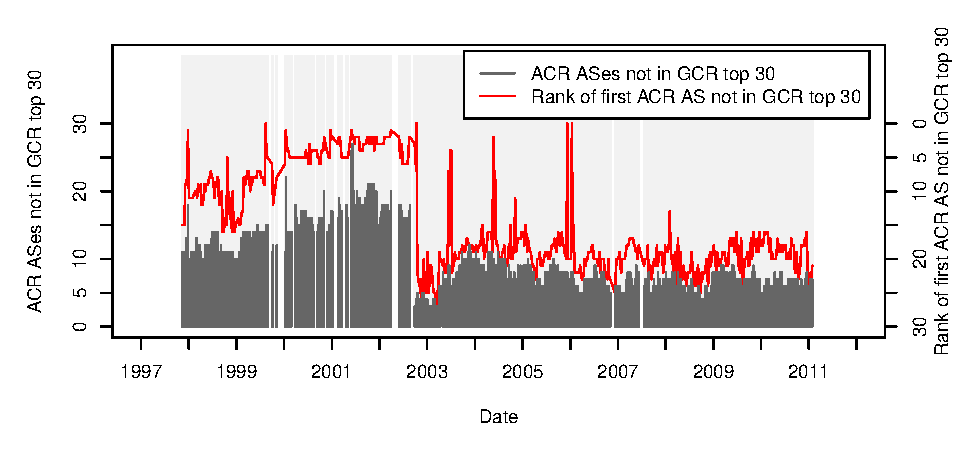
\includegraphics[width=6in]{figures/cidr_report_validity_top30_error.pdf}
%     \vspace{-2em}\\
%     \caption{The number and first rank of ASes in the treatment group (top 30)
%         of the ACR that are not in the treatment group of the GCR over time.}
%     \label{fig:comp_top30_error}
% \end{singlespace}
% \end{centering}
% \end{figure}

It was difficult to develop an implementation of the CIDR Report aggregation
algorithm (which is used to produce the GCR) that exactly matches the output of
the authoritative CIDR Report. Further, it is questionable whether an
implementation of the algorithm should strive to reproduce the output of a
``black box'' (even if it is the black box that is used to inform and influence
the operator community) instead of being based on first principles and a
conceptual understanding of the purpose of the CIDR Report. Given that our
implementation was developed on the basis of the principles of route
aggregation, along with the fact that the GCR is reasonably in agreement with
the ACR, we believe it is reasonable to use this data in our analysis.

\section{Characteristics of the CIDR Report}

In analyzing the CIDR Report, much time was spent looking at characteristics of
the report and networks that appear on it. While this was not directly related
to answering the question of whether appearing on the CIDR Report changes route
aggregation behavior, it is useful in providing context about the CIDR Report,
and also possibly offering insights about why the Report was or was not
effective, or how its efficacy may have changed over time. The characteristics
discussed in this section are organized into two categories: relative measures
of network behavior on the CIDR Report (typically related to ranks and ranking)
and absolute measures of network behavior (typically related to prefixes
advertised).

\subsection{AS appearances and rank-based observations}
The first approach taken to gain an understanding of the behavior of the CIDR
Report was to visualize it in a two-dimensional space, with time in one
dimension and CIDR Report rank in the other dimension. An excerpt of this
visualization is shown in Figure \ref{fig:viz_sample}.

\begin{figure}[h!]
\begin{centering}
\begin{singlespace}
    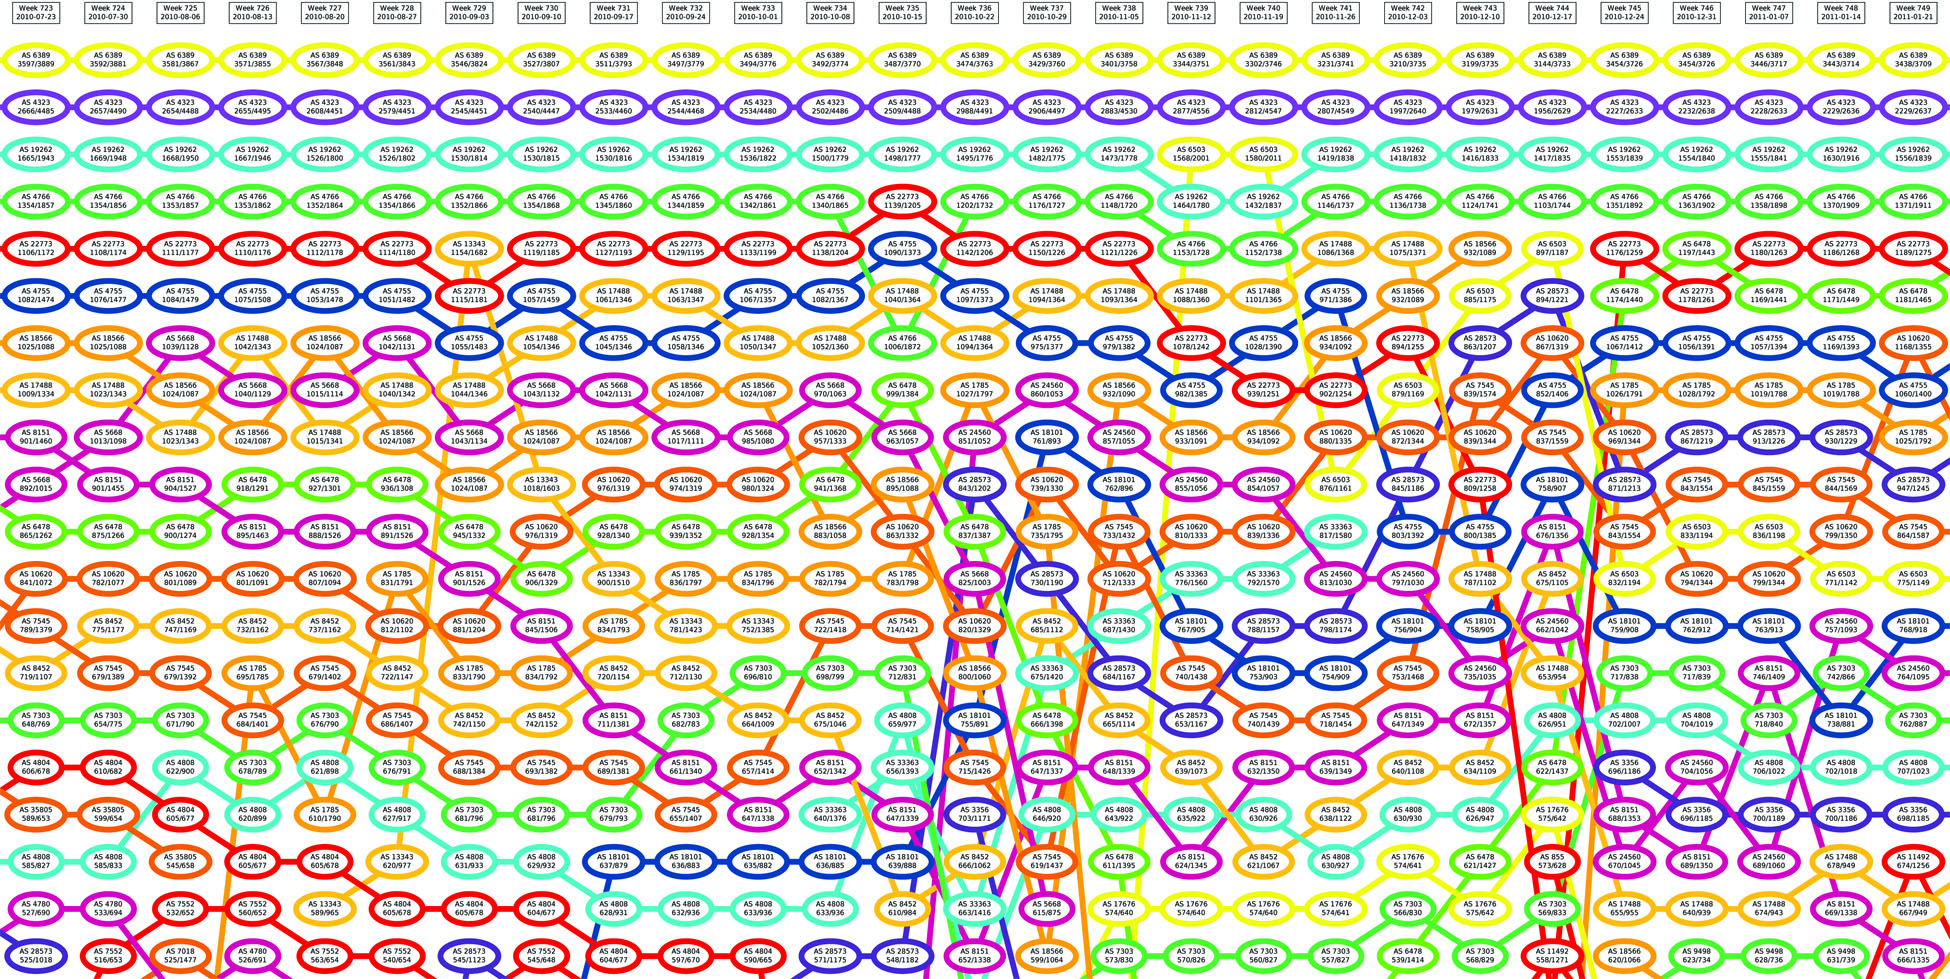
\includegraphics[width=4in]{figures/viz_sample.jpg}
    \caption{A sample of our CIDR Report visualization.}
    \label{fig:viz_sample}
\end{singlespace}
\end{centering}
\end{figure}

This visualization was not especially practical, as it was physically large and
the level of detail and limited range of colors available made it difficult to
visually identify and distinguish the behaviors of individual ASes. However,
this visualization provided some hints regarding interesting characteristics to
investigate. By visual inspection, it appeared as though the CIDR Report was
volatile at lower ranks but relatively static near the top (ASes with the most
aggregation potential). It also appeared that the report was more volatile in
the past but become more static overall more recently. These and other aspects
were then investigated using analytic techniques, which are described and
presented next.

A number of interesting characteristics about the CIDR Report are of a
demographic nature, such as how many ASes appear on the CIDR report, or for how
long do ASes remain on the report? This first question, about how many ASes
ever appear on the CIDR Report, is illuminated by Figure \ref{fig:as_counts}.

\begin{figure}[h!]
\begin{centering}
\begin{singlespace}
    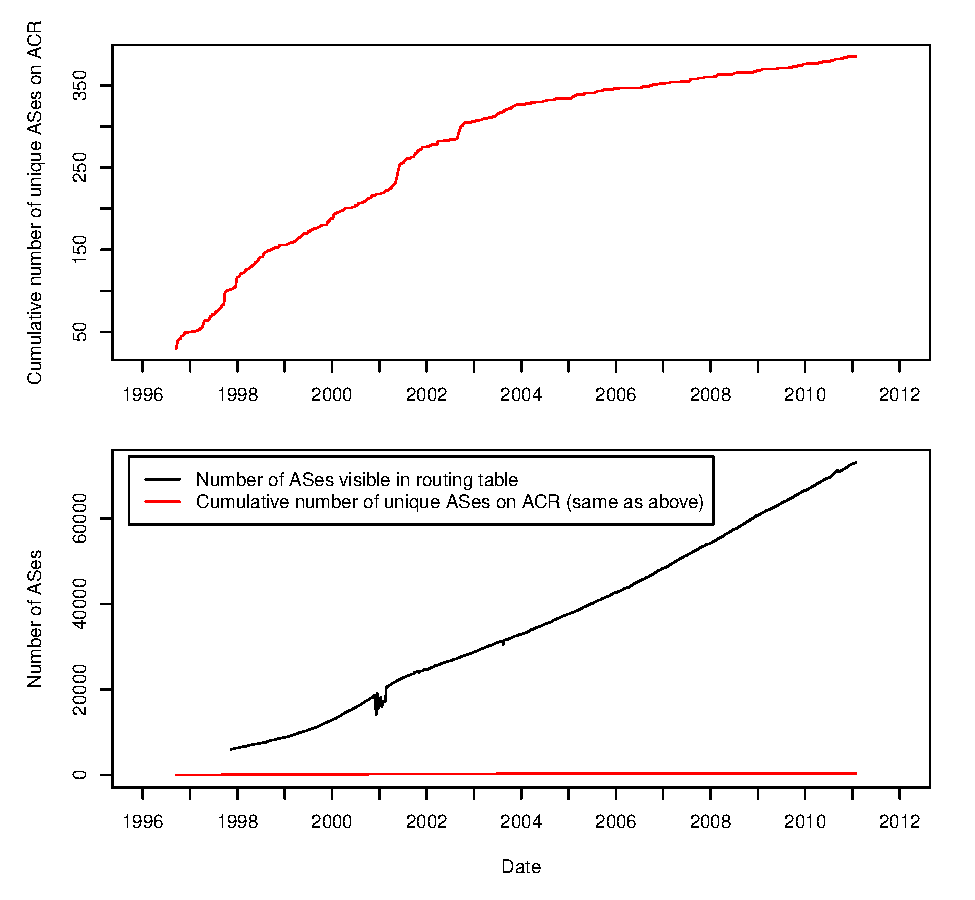
\includegraphics[width=6in]{figures/cumulative_asn_counts.pdf}
    \vspace{-2em}\\
    \caption[A cumulative count of the unique ASes that have appeared on the
        CIDR Report]{A cumulative count of the unique ASes that have appeared
        on the CIDR Report and compared to the cumulative count of unique ASes
        visible in the routing table up to the same point.}
    \label{fig:as_counts}
    %TODO: in future, think about plotting unique ASes ever appearing within
    %certain rank slots.
\end{singlespace}
\end{centering}
\end{figure}

In this figure, the top plot shows the cumulative number of ASes that appear on
the CIDR Report, starting with 30 ASes on the first report in 1996 and
concluding with 386 unique ASes in 2011. The growth of new ASes appearing on
the report appears to be greater in the late 1990s and early 2000s than in the
mid-late 2000s. More remarkable is how relatively few ASes from the total set
of ASes that ever appear in the Internet routing table appear on the CIDR
Report. This relationship is shown in the bottom plot of Figure
\ref{fig:as_counts}. In this figure, the red curve near the bottom of the graph
area is the same red curve that was plotted in the upper figure, and the black
curve that rises steadily is the total number of ASes visible in the routing
table. This illustrates that less than 1\% of all ASes have ever appeared on
the CIDR Report.

While the former plot illustrated the total number of ASes that appear on the
report, it does not provide any information about how long an AS appears on the
report. This information is provided in the next figure, Figure
\ref{fig:cdf_weeks}, which presents a cumulative distribution function of the
total number of weeks each AS appears on the CIDR Report. Noting the log scaled
x-axis, we can see that 15\% of all ASes that appear on the CIDR Report
are on the report for only a single week, half of all ASes are on the report
for approximately 10 weeks or less, and that there is a general exponential
relationship between increasing fractions of the population and time spent on
the report (i.e. for each 10\% increase in population considered, the maximum
duration spent on the report doubles).

\begin{figure}[h!]
\begin{centering}
\begin{singlespace}
    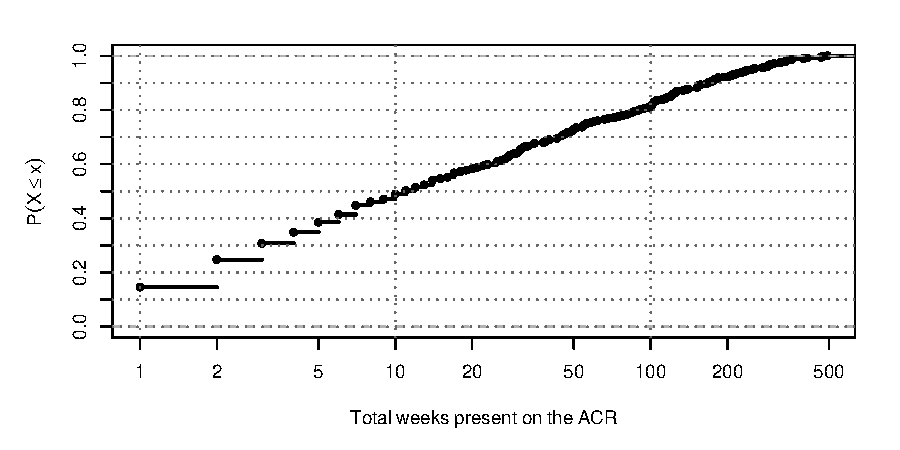
\includegraphics[width=6in]{figures/acr_cdf_weeks.pdf}
    \vspace{-2em}\\
    \caption{A CDF of the total number of weeks that each AS is visible on the
    CIDR Report.}
    \label{fig:cdf_weeks}
\end{singlespace}
\end{centering}
\end{figure}

%TODO: tempting to take the following graf and figure out.
% A similar plot with a different metric is shown in Figure
% \ref{fig:cdf_rankweeks}. In this figure, instead of presenting the number of
% weeks each AS spends on the report, the number of rank-weeks accrued by each AS
% are displayed instead. A rank week is simply the sum of the ranks an AS
% occupies for each week it appears on the CIDR Report. So an AS could accumulate
% a rank-week measure of 100 by spending 100 weeks at the very bottom of the
% report (rank of 1, 30th position) or 10 weeks at a rank of 10 (20th position).
%
% \begin{figure}[h!]
% \begin{centering}
% \begin{singlespace}
%     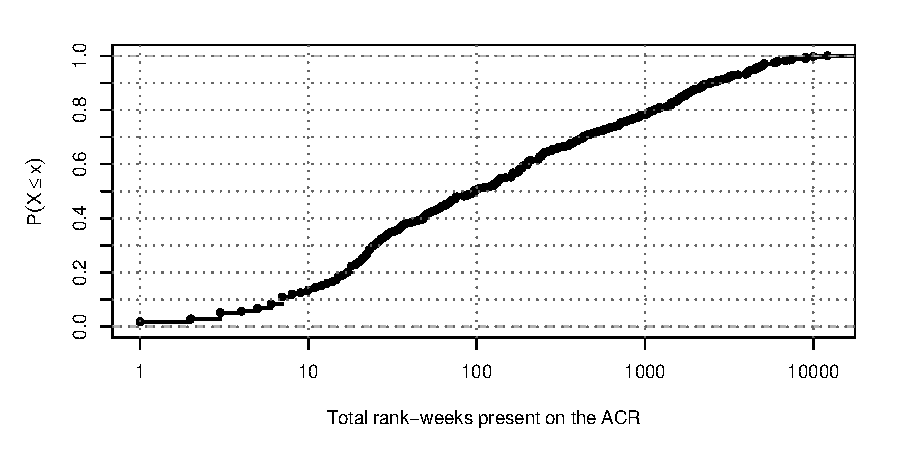
\includegraphics[width=6in]{figures/acr_cdf_rankweeks.pdf}
%     \vspace{-2em}\\
%     \caption{A cumulative distribution function of the total number of
%         rank-weeks that each AS is visible on the CIDR Report.}
%     \label{fig:cdf_rankweeks}
% \end{singlespace}
% \end{centering}
% \end{figure}

This is the first indication that not all the ASes that appear on the CIDR
report behave in similar ways, but instead that many ASes appear on the Report
only briefly in comparison to some ASes that spend a considerable duration of
time on the CIDR Report.

% \begin{figure}[H]
% \begin{centering}
% \begin{singlespace}
%     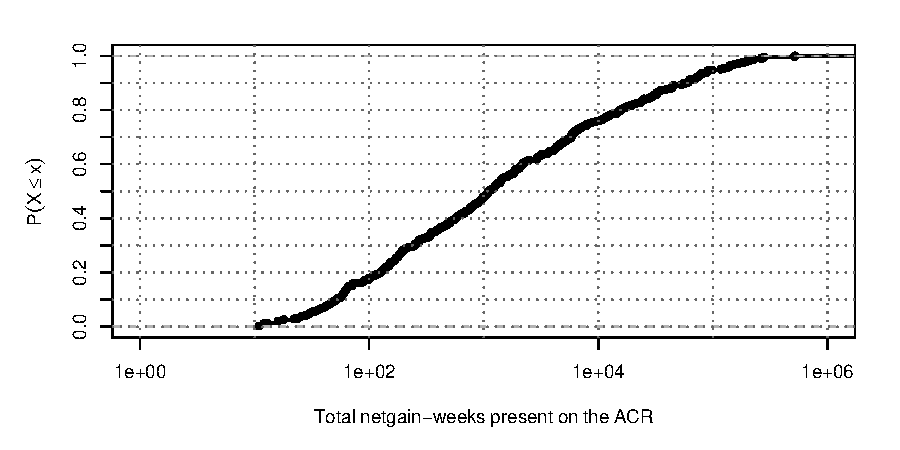
\includegraphics[width=6in]{figures/acr_cdf_ngweeks.pdf}
%     \vspace{-2em}\\
%     \caption{A cumulative distribution function of the total number of netgain-weeks that each AS is visible on the CIDR Report.}
% \end{singlespace}
% \end{centering}
% \end{figure}

Returning to the observation from earlier that the top ranks of the CIDR Report
are more static relative to the volatile lower ranks, we investigate this
further by plotting cumulative distribution functions of the number of weeks
that a particular AS occupies a given rank on the CIDR Report. These plots, for
ranks 1 (most potential for aggregation) to 30, are shown in groups in Figure
\ref{fig:rank_cdfs}

\begin{figure}[h!]
\begin{centering}
\begin{singlespace}
    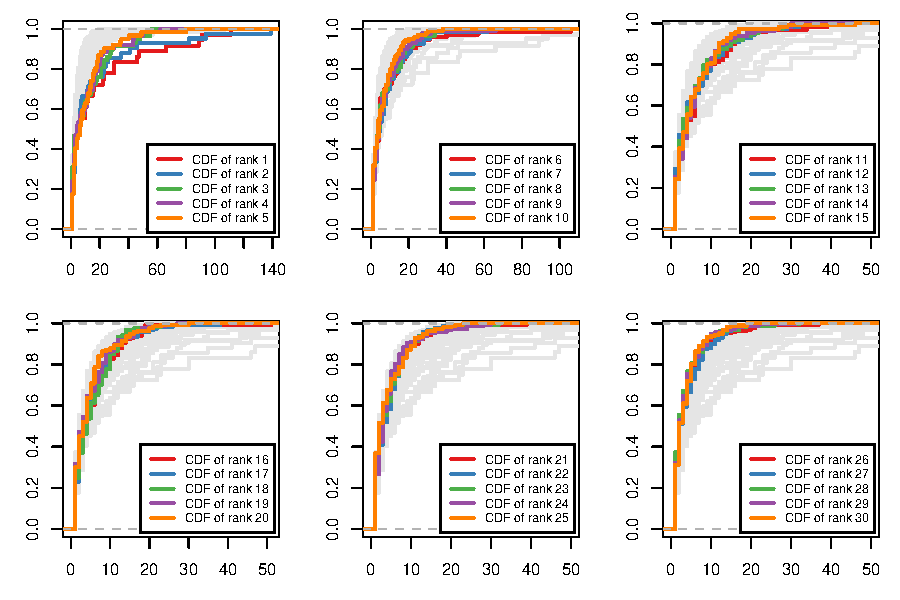
\includegraphics[width=6in]{figures/cr_rank_cdfs.pdf}
    \vspace{-2em}\\
    \caption[CDFs of the number of weeks that a given rank was occupied by a
    single AS]{CDFs of the number of weeks that a given rank was occupied by a
    single AS. The x-axis is the number of weeks, and the y-axis is the
    fraction of the population. The light gray lines indicate CDFs of other
    ranks, in order to place the highlighted ranks in context.}
    \label{fig:rank_cdfs}
\end{singlespace}
\end{centering}
\end{figure}

As illustrated clearly by this figure, lower ranks on the CIDR Report are more
volatile than top ranks. The top five positions, ranks 1-5, are particularly
ossified, with the top 10\% of ASes that ever appear occupying individual ranks
for no less than 20-60 weeks. In contrast, the lower ranks, and particularly
the bottom half (ranks lower than 15) are much more volatile, with around
90\% of the AS population occupying a given rank for 10 weeks or less, and
essentially all of the population not occupying ranks for more than 20
weeks. This is consistent with the claimed observation of operators that
the CIDR Report does not appear to change much---especially the top ranks
that are first visible in the email. The apparent reason for this ossification
will be discussed in the next section.

\subsection{Prefix-based observations}

%TODO: include a figure of the proportion of the routing table that is
%aggregable/deaggregated over time? Plot deagg_factor or frac_aggr?

While the previous section presented interesting observations about AS
appearances and volatility on the CIDR Report, it was focused on the relative
measures of AS rank and appearance within the top 30 on the CIDR Report. It is
also helpful to gain a perspective about characteristics of the CIDR report
considering the number of prefixes that each AS is advertising, as prefix
counts (and routing table slots) are ultimately the metric that is important in
considering behavior change in the context of the routing table.

Figure \ref{fig:netcompare}\footnote{All data in this plot is from the GCR, but
classification of an AS and its netgain/netsnow figures are based on the ASes
present on the ACR as emailed. Data from the GCR is used to allow for
consistent comparison between the entire routing table and the top 30 (ACR)
ASes.} illustrates the fraction of the the total prefixes and aggregable
prefixes visible in the Internet routing table that are advertised by ASes
appearing on the CIDR Report.

\begin{figure}[h!]
\begin{centering}
\begin{singlespace}
    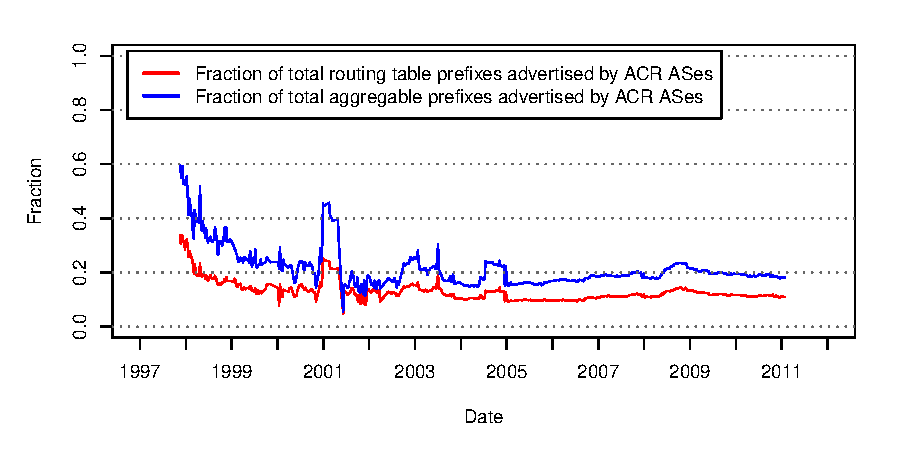
\includegraphics[width=6in]{figures/acr_gcr_netcompare2.pdf}
    \vspace{-2em}\\
    \caption{The fractions of total prefixes and total aggregable
    prefixes in the routing table that are advertised by ASes appearing on the
    CIDR Report.}
    \label{fig:netcompare}
\end{singlespace}
\end{centering}
\end{figure}

This figure suggests that, in the past, the CIDR Report did focus quite
effectively on most of the ``worst offenders'' in terms of networks advertising
aggregable routes. At the beginning of the period of available data, the Report
captured nearly 60\% of the total aggregable routes in the top 30 list. This
has decreased but, interestingly, remained approximately proportional to the
growth of the routing table since 2003 or 2004, suggesting that growth of
deaggregation in the ASes at the top of the CIDR Report is proportional to the
growth of deaggregation across the Internet routing table. However, as the next
figure will show, this proportionality has been maintained in the face of
growth of the number of participants in the Internet routing table, such that
the ASes that appear at the top of the report have become outliers compared to
most of the ASes in the routing table.

Another way of considering how the prefix advertisement behaviors of networks
on the CIDR Report compares to the other networks in the routing table is to
look at the distribution of deaggregation (advertisement of aggregable
prefixes) in the routing table. Cumulative distribution functions of aggregable
prefixes (netgain) visible in the routing table (from the GCR) over time is
shown in Figure \ref{fig:netgain_cdf}.

% TODO in future, look into whether the distribution of deaggregators is a
% power-law relationship
\begin{figure}[h!]
\begin{centering}
\begin{singlespace}
    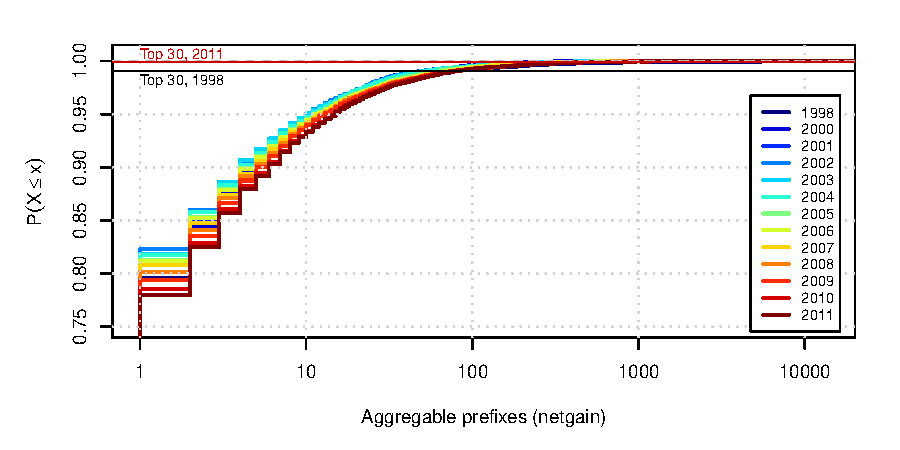
\includegraphics[width=6in]{figures/netgain_cdf_gcr.pdf}
    \vspace{-2em}\\
    \caption[CDFs of netgain of all ASes in the routing table in the first week
    of the year from 1998-2011]{CDFs of netgain of all ASes in the routing
    table in the first week of the year from 1998-2011. Threshold lines
    indicating the cut-off point for appearing on the CIDR Report in 1998 and
    2011 are indicated. Note that the graph is rescaled; approximately 70\% of
    ASes in the routing table do not advertise any aggregable prefixes.}
    \label{fig:netgain_cdf}
\end{singlespace}
\end{centering}
\end{figure}

From these distributions we can see that while advertisement of aggregable
prefixes has increased slightly across the routing table over time, as given by
the downward movement of the CDF curves over time, the distribution of
aggregable prefixes announced by ASes has remained roughly similar, with an
increasingly long tail of outliers in the top fraction of a percentile of
the population of ASes. This figure is potentially misleading, as while the
distribution of aggregable prefix announcement has not changed, the total
number of ASes visible in the routing table has grown over time, from 3172 ASes
in the first week of 1998 to 36383 ASes in the first week of 2011. Thus, there
are now approximately ten times as many ASes announcing a given number of
aggregable prefixes as there were in 1998.

What is also noteworthy in this figure is the indication of the threshold
points for appearing on the CIDR Report in 1998 and 2011. The fraction of the
population above this line is the ``top 30'' group that would appear on the
CIDR Report. This line appears to have moved from approximately 1\% of the
population in 1998 to some small fraction of a percent in 2011. This conclusion
follows from the fact that the number of ASes in the routing table has grown
over time and yet the ``top 30'' threshold of the CIDR report has remained
constant. However, as this figure, as well as Figure \ref{fig:netcompare}
illustrate, this also means that the CIDR Report has changed to highlight
mostly outlier behavior, leaving the individually less significant but
collectively more significant deaggregation below the threshold unaddressed.

% \begin{figure}[H]
% \begin{centering}
% \begin{singlespace}
%     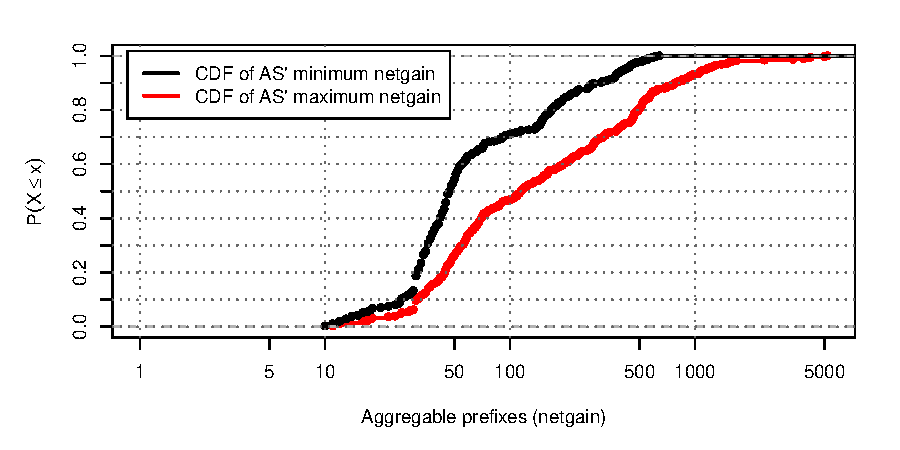
\includegraphics[width=6in]{figures/acr_netgain_cdfs.pdf}
%     \vspace{-2em}\\
%     \caption{CDFs of the minimum and maximum netgain observed for each AS during its time on the CIDR Report.}
% \end{singlespace}
% \end{centering}
% \end{figure}

The question of where the threshold to appear on the CIDR Report is in terms of
netgain---how much deaggregation it takes for an AS to appear on the
report---is addressed in Figure \ref{fig:thresholds}. This figure displays the
minimum netgain thresholds to appear on the CIDR Report (rank 30) as well as
the median (rank 15) and various other top ranks.

\begin{figure}[h!]
\begin{centering}
\begin{singlespace}
    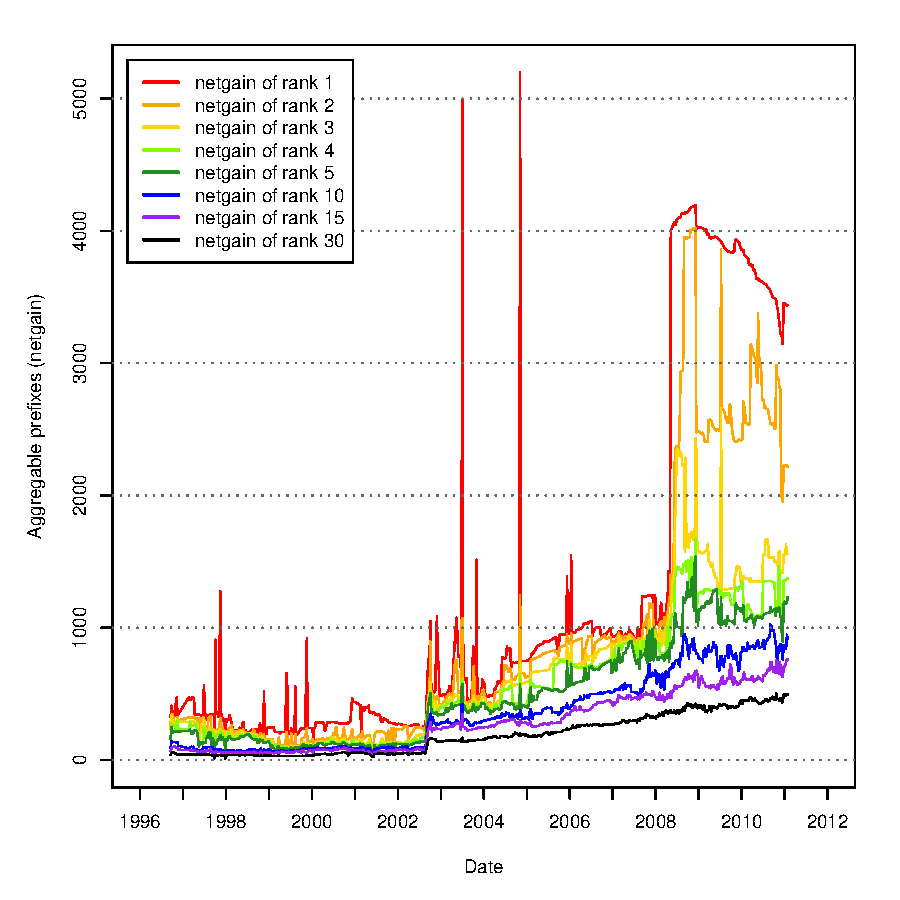
\includegraphics[width=6in]{figures/acr_netgain_time.pdf}
    \vspace{-2em}\\
    \caption{Netgain thresholds required to achieve indicated ranks on the ACR
    over time.}
    \label{fig:thresholds}
    \end{singlespace}
\end{centering}
\end{figure}

% Anyone who can deaggregate a /15 can get on the CIDR Report -- how many of
% these folks are there? ARIN Bulk WHOIS

This figure of the CIDR Report rank thresholds shows an increasing spread in
prefix thresholds for the various ranks over time, particularly in the top 5,
as well as between the top 5 and the median, compared to between the median and
the minimum threshold (rank 30). The increasing spread between ranks can also
be viewed in a slightly different way, with a focus on temporal progression, in
the following figure.

Figure \ref{fig:netgain_cdf_acr} presents cumulative
distribution functions of the number of aggregable prefixes (netgain)
advertised by each AS on the ACR in the first week of the year indicated.

\begin{figure}[h!]
\begin{centering}
\begin{singlespace}
    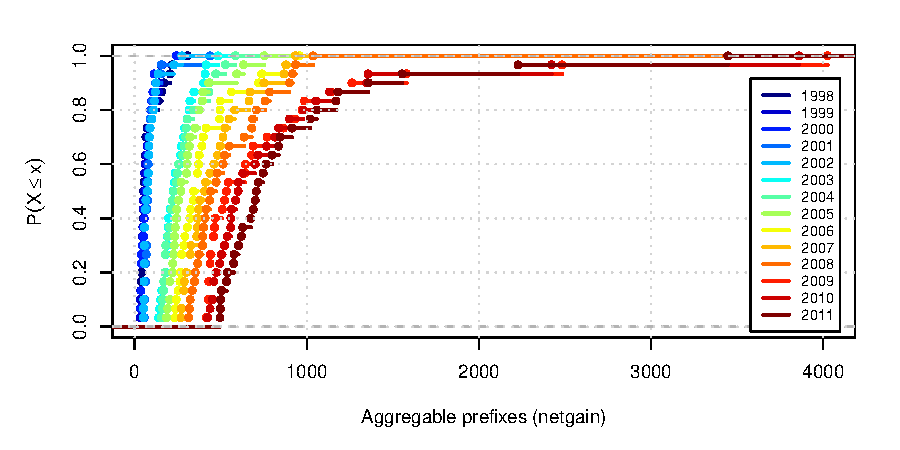
\includegraphics[width=6in]{figures/netgain_cdf_acr.pdf}
    \vspace{-2em}\\
    \caption[CDFs of the netgain of the ASes visible on the ACR in the first
    week of each year 1998-2011]{CDFs of the netgain of the ASes visible on the
    ACR in the first week of each year 1998-2011. Notice that the top of the
    population spreads more in later years.}
    \label{fig:netgain_cdf_acr}
\end{singlespace}
\end{centering}
\end{figure}

Here again we see the growing spread between ranks and the changing shape of
the distribution as ASes at the top of the report announce increasingly more
aggregable prefixes in later years than in previous years. Both this figure and
the previous figure suggest that the ossification in the top ranks of the CIDR
report observed earlier are due to the growing spread in netgain, making it
more difficult to ``unseat'' high-ranked ASes because they are so far from the
next nearest AS (in terms of number of prefixes). This is not necessary a
problem, and also our measure of volatility may be imperfect (i.e. an AS could
oscillate between two ranks, appearing volatile even though its behavior does
not chance perceptibly), but this does provide some explanation for the static
behavior noted before.

% Finally, just because it is interesting, I include a plot of the minimum
% threshold, in terms of aggregable prefixes, that are necessary to appear on the
% CIDR Report over time.
%
% %TODO should I include this???
% \begin{figure}[H]
% \begin{centering}
% \begin{singlespace}
%     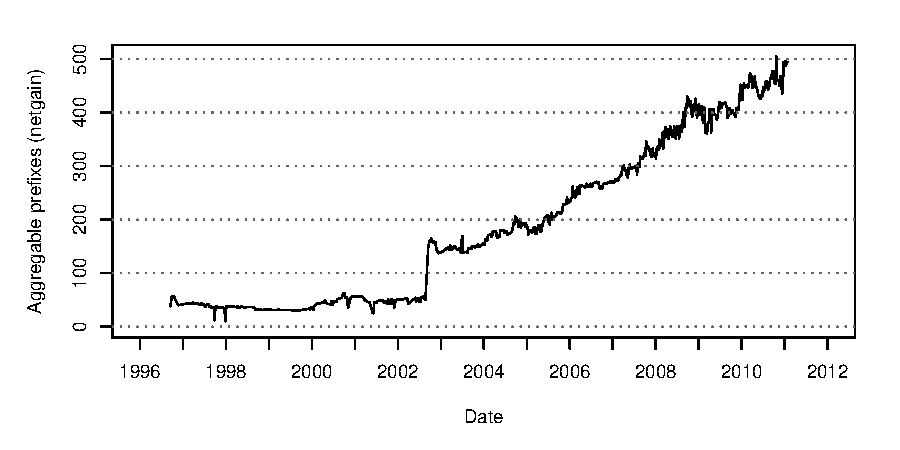
\includegraphics[width=6in]{figures/acr_netgain_time_min.pdf}
%     \vspace{-2em}\\
%     \caption{A plot of the minimum netgain required to appear on the CIDR
%     Report over time.}
%     \end{singlespace}
% \end{centering}
% \end{figure}

%TODO should I include this???
% \begin{figure}[h!]
% \begin{centering}
% \begin{singlespace}
%     \includegraphics[width=6in]{figures/netgain_frac_aggr_cdf_gcr.pdf}
%     \vspace{-2em}\\
%     \caption{Plots of CDFs of the fraction of prefixes announced by each AS
%     that are aggregable, over time.}
%     \label{fig:netgain_cdf_acr}
% \end{singlespace}
% \end{centering}
% \end{figure}

\subsection{Conclusions}

Our observations of characteristics of the CIDR Report related to the number of
prefixes advertised by each AS, as well as the previous observations about the
rank of each AS and appearance of ASes on the CIDR Report, suggest that while
the advertisement of redundant, aggregable prefixes in the routing table is
reasonably commonplace, the ASes that appear on the CIDR Report are outliers in
that they announce significantly more aggregable prefixes than most of the rest
of the population of ASes participating in the interdomain routing system. In
its earlier days the CIDR Report captured a larger fraction of the ASes
responsible for aggregable prefixes than it does now, because of growth in the
total number of ASes participating in the Internet and announcing aggregable
routes. The top of the Report has become relatively static because of the
extreme deaggregation of ASes at the top of the report relative to the majority
of the AS population.

\section{Analysis of AS behavior after appearing on the CIDR Report}

This section presents and discusses the results of the primary question of this
thesis: \emph{do autonomous systems change their behavior, as measured by the
number of aggregable routes they advertise into the routing table (netgain),
after appearing on the CIDR Report?} As described in section
\ref{sec:method_agg_report_analysis}, data from the CIDR Report is processed to
determine when ASes first appear on the report, and samples are then taken from
30 to 730 days after this initial appearance (detailed in Figure
\ref{fig:sample_ex}) and compared to the value at the time of first appearance.
Decreases in netgain would suggest that the CIDR Report does influence network
operator route aggregation behavior in the expected or intended way, while no
change or increased netgain would suggest that the CIDR Report has no effect.
The group of ASes appearing on the CIDR Report, and thus theoretically subject
to social forces to improve aggregation behavior, will hereafter be referred to
as the treatment group.

In an attempt to control for normal variation in AS behavior that does not
result from appearing on the CIDR Report, a ``control group'' was established
from ASes never appearing on the CIDR Report, as described in much more detail
in section \ref{sec:method_agg_report_analysis}. While this group will be
referred to as the control group, it is more precisely the ``untreated group'',
given that this is a quasi-experiment instead of a randomized, controlled
experiment.

We measure and present three quantities in an effort to discern the behavior of
ASes appearing on the CIDR Report. The first two, absolute and relative change
in netgain ($\Delta\textrm{netgain}$), measure directly the change in the
number of aggregable prefixes announced by an AS after appearing on the CIDR
Report. The third measure, deaggregation factor (DF), is the ratio of the total
number of prefixes announced by an AS to the minimum number of prefixes
required to be announced by the same AS in order to implement the same routing
policy with perfect aggregation. Unlike netgain, DF is a relative measure of
deaggregation, and considers deaggregation in proportion to the total number of
prefixes a network operator must announce to operate their network. The
operational definition of DF will be described in its respective section.

All of the figures that will be presented next are a series of cumulative
distribution functions (CDFs) of the quantity of interest at different periods
after an AS' initial appearance on the CIDR Report. In general, these CDFs can
be interpreted as that the ASes in the group improved their aggregation
behavior if the curve appears to move upwards or towards the left of the $x=0$
line over time. This indicates a greater fraction of the population has reduced
its advertised prefixes. While specific issues of interpretation for each plot
will be discussed as appropriate in the relevant sections below, this is a very
rough rule of thumb for thinking about the figures that will now follow.

With this initial explanation, we are ready to present the results of our
analysis, beginning with netgain and followed with deaggregation factor, which
most clearly associates a change in aggregation behavior with an appearance on
the CIDR Report. Unless otherwise noted in captions of the figures or the
associated text, all of the following figures utilize all appearances on the
CIDR Report from 1997-2011. Additional figures of these quantities utilizing
appearances from only a portion of the date range, to discern changes in
behavior over time, are included in Appendix \ref{chap:additional_figs}.

\subsection{Change in netgain following CIDR Report appearance}

Netgain, the number of aggregable prefixes advertised by an AS, was the first
measure we examined for behavior change in response to appearing on the CIDR
Report. This seemed to be a reasonable first measure as this is the quantity
most clearly of interest with regard to routing table size and the CIDR Report.
Cumulative distribution functions of changes in netgain following appearance on
the CIDR Report, and a corresponding untreated control group is shown below in
Figure \ref{fig:delta_netgain_cdf}. Change in netgain is defined as
$\Delta\textrm{netgain}_{t+k} = \textrm{netgain}_{t+k} -
\textrm{netgain}_{t+0}$, where $t$ is symbolic of the time of first appearance,
and $k$ is one of the measurement time periods from 30-730 days

\begin{figure}[h!]
\begin{centering}
\begin{singlespace}
    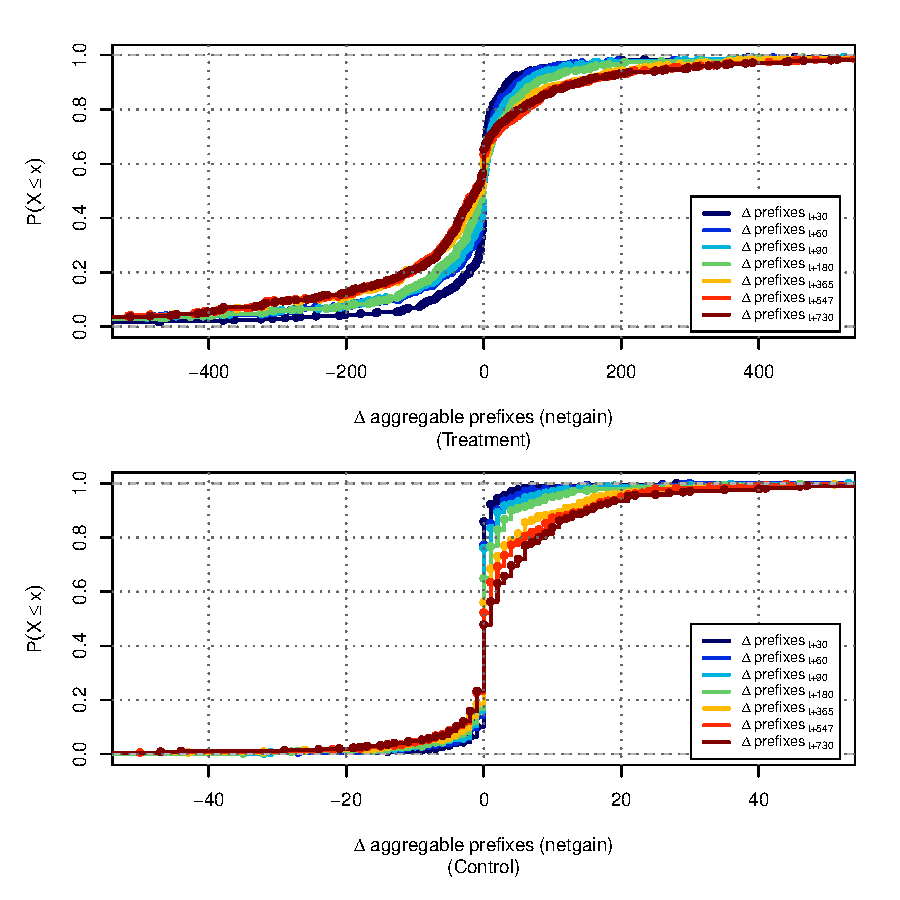
\includegraphics[width=6in]{figures/behavior-netgain-1997_2011-corr.pdf}
    \vspace{-2em}\\
    \caption{CDFs of change in number of aggregable prefixes (netgain)
    advertised by treated and untreated (control) ASes, for the period
    1997-2011.}
    \label{fig:delta_netgain_cdf}
\end{singlespace}
\end{centering}
\end{figure}

From the top plot in this figure, we can observe that slightly more than half
(60\%) of the AS appearances on the CIDR Report were followed by a decrease in
aggregation or no further deaggregation. It also shows that, in an absolute
sense, there is a greater reduction in aggregable routes than advertisement of
new aggregable routes (i.e. the most-reducing 10\% reduce by approximately 200
prefixes or more, whereas the most-increasing 10\% increase by approximately 50
prefixes or more) with the exception of outliers. There are still significant
outliers on both sides, and this plot is trimmed to exclude them.

In contrast to the treatment group, the control group shown in the bottom
figure exhibits different behavior, with approximately half of the population
exhibiting increased announcement of aggregable prefixes, while only 20\% of
the population decreased announcement of aggregable prefixes. Further, the
absolute amount of increased deaggregation is more significant than the amount
of reduced deaggregation.

While absolute measures are ultimately the metric of interest with regard to
our concern about the size of the routing table and the number of slots used by
each AS, they are less useful to determine the significance of increased or
decreased aggregation relative to an AS' initial behavior. Thus, we present
CDFs of the relative change in netgain
($\Delta\textrm{netgain}_{t+k}/\textrm{netgain}_{t+0}$) in Figure
\ref{fig:delta_rel_netgain_cdf}. This figure is essentially a normalized
version of Figure \ref{fig:delta_netgain_cdf}.

\begin{figure}[h!]
\begin{centering}
\begin{singlespace}
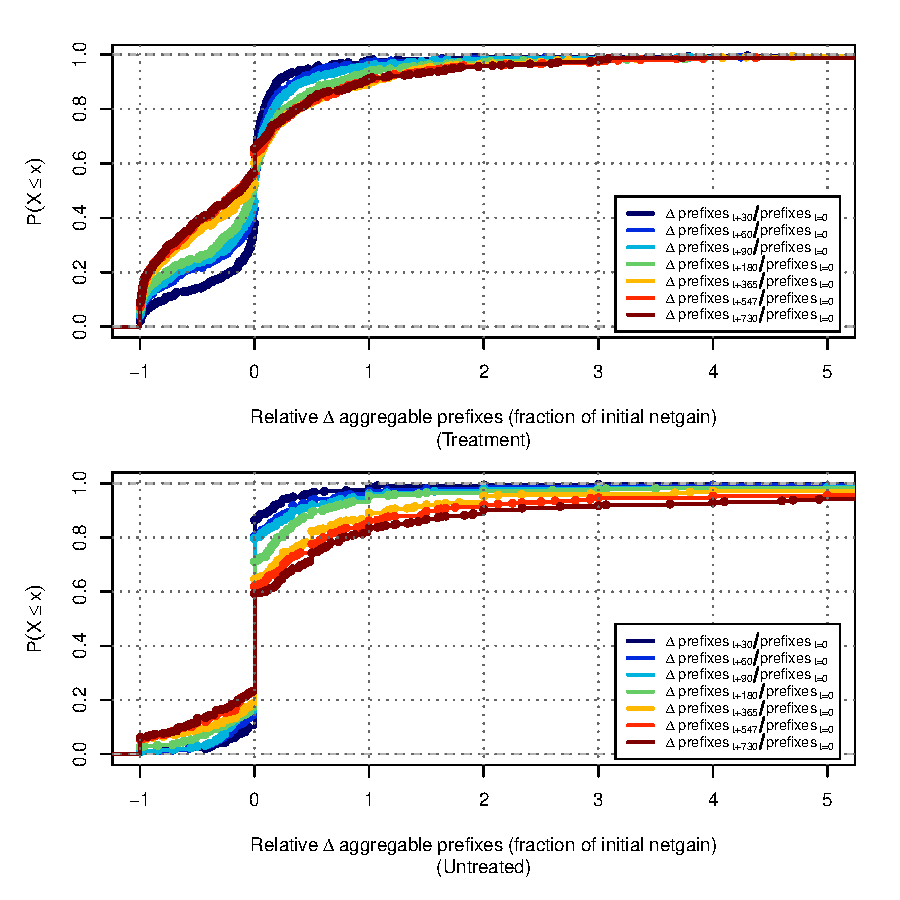
\includegraphics[width=6in]{figures/behavior-rel_netgain-1997_2011-corr.pdf}
    \vspace{-2em}\\
    \caption{CDFs of relative change in number of aggregable prefixes (netgain)
    advertised by treated and untreated (control) ASes, for the period
    1997-2011.}
    \label{fig:delta_rel_netgain_cdf}
\end{singlespace}
\end{centering}
\end{figure}

This figure makes it easier to quantify the change in netgain over time. By 730
days, approximately 20\% of the population have nearly fully aggregated,
another 20\% have reduced deaggregation by 50\% or more, and a third 20\% have
held steady or reduced aggregable routes by less than 50\%. In contrast,
another 20\% have approximately increased deaggregation by up to 50\%, and the
top 10\% increased deaggregation by 100\% or more. As noted in the previous
figure, improvements in deaggregation are much less pronounced in the control
group.

There appears to be a small amount of significant aggregation in
the first measurement period after a CIDR Report appearance, and can be seen
by looking at the $t+30$ curve on the treatment plot above. Thirty days after
appearing on the report, approximately 10\% of ASes improved aggregation by at
least 50\%. While there was also some movement towards further deaggregation at
the top of the plot, perhaps approximately 5\% of the population deaggregated
by at least 50\%, with much more of the population remaining near the $x=0$
line, indicating little change in behavior.
% Perhaps more interesting is that changes leading to reduction in
% deaggregation initially occur more quickly than changes leading to increased
% deaggreation.  This can be seen by looking at the shape of the CDF plot over
% time, noting that

% \subsection{Change in netsnow in response to CIDR Report appearance}
%
% \fbox{NOTE TO Karen and Dave:}
% I decided to leave this section and corresponding figures out, as I don't
% think they add much.
%
% \begin{figure}[H]
% \begin{centering}
% \begin{singlespace}
%     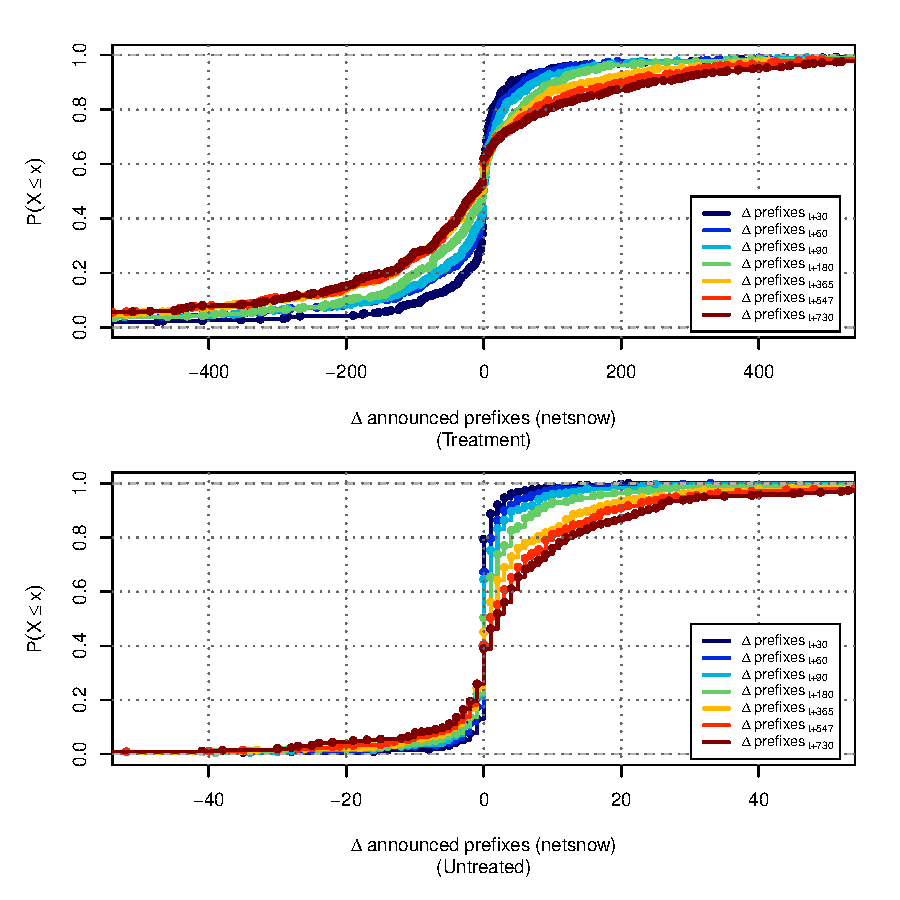
\includegraphics[width=6in]{figures/behavior-netsnow-1997_2011-corr.pdf}
%     \vspace{-2em}\\
%     \caption{Cumulative distribution function of change in total number of
%     prefixes (netsnow) advertised by treated and untreated (control) ASes, for
%     the period 1997-2011.}
%     \label{fig:delta_netsnow_cdf}
% \end{singlespace}
% \end{centering}
% \end{figure}
%
% \begin{figure}[H]
% \begin{centering}
% \begin{singlespace}
%     \includegraphics[width=6in]
%         {figures/behavior-rel_netsnow-1997_2011-corr.pdf}
%     \vspace{-2em}\\
%     \caption{Cumulative distribution function of relative change in total
%     number of prefixes (netsnow) advertised by treated and untreated (control)
%     ASes, for the period 1997-2011.}
%     \label{fig:delta_rel_netsnow_cdf}
% \end{singlespace}
% \end{centering}
% \end{figure}

\subsection{Change in deaggregation factor following CIDR Report appearance}
% \subsection{Change in fraction aggregable in response to CIDR Report
% appearance}

While netgain provides a direct measure of unnecessary prefixes occupying the
routing table, it does not take into account the total size of an AS'
operations or networks, and so an AS announcing 101 prefixes which could be
aggregated into one prefix would receive the same netgain score (100) as an AS
announcing 2000 prefixes that could be aggregated into 1900 prefixes. While it
is true that in an absolute sense, both of these configurations contribute the
same number of unnecessary prefixes to the Internet routing table, the
announcement of a large number of aggregable prefixes relative to one's total
network is arguably less defensible or justifiable than a network that
introduces a relatively small amount of deaggregation as a result of operating
its large network.

To investigate this relative degree of deaggregation, we also measure the
deaggregation factor (DF), the ratio of the current number of prefixes
advertised by an AS to the minimum number of prefixes needed to be advertised
by the same AS to implement their current routing policy with perfect
aggregation\footnote{This configuration is preferable to a seemingly similar
ratio of netgain to netsnow, our original approach, as netsnow is not
independent of netgain:
$\textrm{netgain}/\textrm{netsnow} =
\textrm{netgain}/(\textrm{netsaggr}+\textrm{netgain})$, making it more
difficult to reason about the causes of changes in this quantity.}.
More precisely,
$\textrm{DF}=\textrm{netsnow}_{t+k}/\textrm{netsaggr}_{t+k}$, where
$\textrm{netsaggr}_{t+k}=\textrm{netsnow}_{t+k}-\textrm{netgain}_{t+k}$. $t$ is
symbolic of the time of first appearance, and $k$ is one of the measurement
time periods from 30-730 days. In the above example, the first network would
have a DF of $\textrm{100}/\textrm{1}=\textrm{100}$, and the second would have
a DF of $\textrm{2000}/\textrm{1900}=\textrm{1.05}$. Cumulative distribution
functions of the deaggregation factor for the treatment and control groups is
shown below in Figure \ref{fig:deagg_factor_cdf}. Note that unlike change in
netgain, DF is not measured relative to the original point of appearance on the
CIDR Report, and so must be viewed together with the DF at the original point
of appearance ($t+0$) in order to observe changes in behavior.

%% \begin{figure}[h!]
% \begin{centering}
% \begin{singlespace}
%     \includegraphics[width=6in]
%         {figures/behavior-frac_deagg-1997_2011-corr.pdf}
%     \vspace{-2em}\\
%     \caption{Cumulative distribution function of change in the fraction of
%     prefixes advertised by treated and untreated (control) ASes that can be
%     aggregated without affecting routing policy, for the period 1997-2011.}
%     \label{fig:frac_agg_cdf}
% \end{singlespace}
% \end{centering}
% \end{figure}

\begin{figure}[h!]
\begin{centering}
\begin{singlespace}
    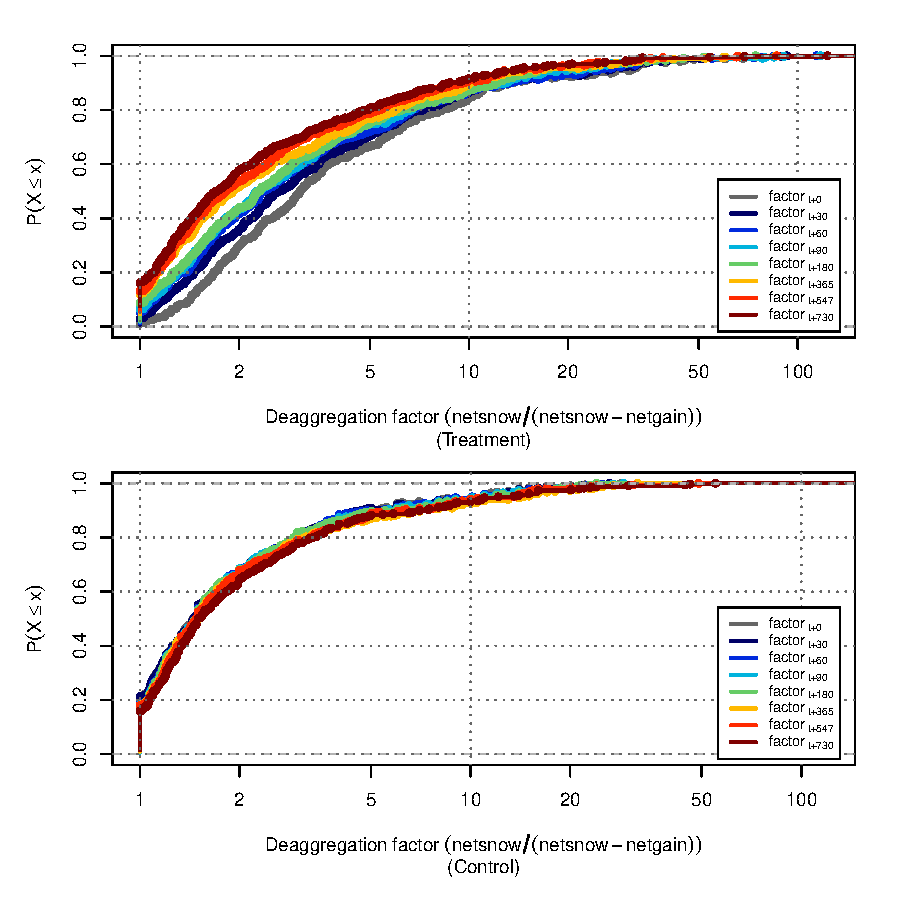
\includegraphics[width=6in]
        {figures/behavior-deagg_factor-1997_2011-corr.pdf}
    \vspace{-2em}\\
    \caption{CDFs of the deaggregation factor for periods of time after an AS
    appears on the CIDR Report (treatment) and for untreated ASes (control),
    for the period 1997-2011.}
    \label{fig:deagg_factor_cdf}
\end{singlespace}
\end{centering}
\end{figure}

This figure suggests a reduction in deaggregation factor following appearance
on the CIDR Report, as indicated by upward movement of the CDF curve along
vertical lines, meaning that a greater fraction of the population has a DF less
or equal to the value at the vertical line than in the previous time period. In
contrast to the treatment group, the control group exhibits little change, and
in fact the change is a slight increase in deaggregation factor over time.

A simplified version of the previous plot, extracting only the first ($t+0$)
and last ($t+730$) measurement, and presenting the curves for the treatment and
control groups together is shown in Figure \ref{fig:deagg_factor_cdf_simple}.
In both cases, the initial measurement is the lighter color, and the latest
measurement is the darker color. 

This figure clearly illustrates the difference in the deaggregation factor of
the ASes that appear on the CIDR Report and those that do not. It also makes it
easier to observe the nature of the change over between initial appearance and
the end of the post-appearance measurement period (two years following the
appearance).

\begin{figure}[H]
\begin{centering}
\begin{singlespace}
    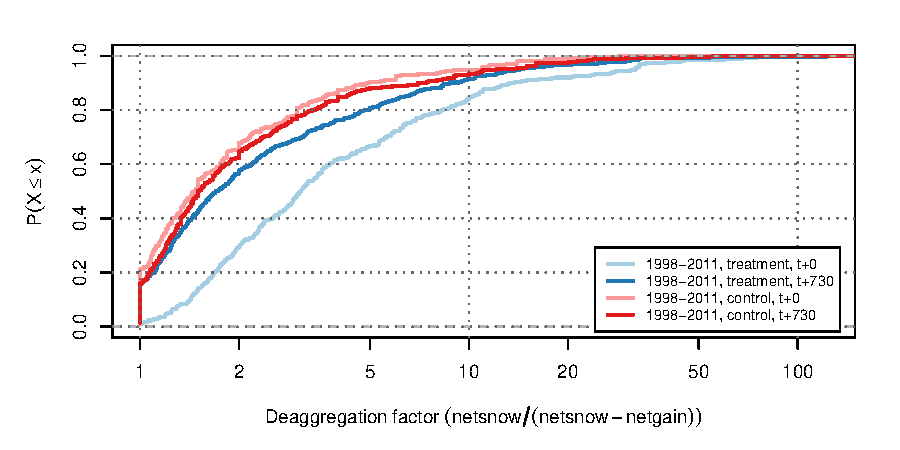
\includegraphics[width=6in]
        {figures/behavior-deagg_factor-1997_2011-special_tc.pdf}
    \vspace{-2em}\\
    \caption{Simplification of previous figure, showing the first (t+0) and
    last (t+730) CDF of the deaggregation factor for both the treatment and
    control groups.}
    \label{fig:deagg_factor_cdf_simple}
\end{singlespace}
\end{centering}
\end{figure}

There is a question here about what exactly this change means, as a reduction
in the deaggregation factor can be caused by one of two changes in an AS'
behavior: a decrease in netgain or an increase in netsaggr (which would result
from increased advertisement of non-aggregable prefixes, presumably from new
address blocks). Looking back at the previous netgain figures, it is certain
that some of this reduction in DF is due to reduction in netgain, though it may
also result from ISPs growing their networks and bringing on new customers. The
latter is an inevitable force in the commercial Internet, and while not
directly encouraged by the CIDR Report (netgain will remain the same), growth
of networks with a reduction in DF is still an improvement relative to growth
with proportional deaggregation.

%TODO: the CIDR Report doesn't treat DF, it treats netgain!!!
%TODO: in an ideal world, plot delta netaggr over time

Since deaggregation factor appears to be a reasonable measure (and that clearly
indicates some behavior change), we will use this measure to investigate the
change in treatment effect of appearing on the CIDR Report over time. To do so,
we will consider the behavior of this measure for a number of smaller time
periods within the overall period for which we have data. This will allow
the observation of any changes in behavior over the course of the available
data. A window of three years was selected and the data set was divided into
four three-year blocks, starting at the beginning of the first year and ending
at the end of the last year: 1998-2000, 2001-2003, 2004-2006, and 2007-2009.
Any appearances on the CIDR Report occurring in these three-year windows were
analyzed and suitable untreated ASes were selected as controls, exactly as
before. Plots for these time periods are shown in Figure
\ref{fig:deagg_factor_cdf_time} (similar figures for observing change in
relative netgain over time are available in Appendix
\ref{chap:additional_figs}).

\begin{figure}[h!]
\begin{centering}
\begin{singlespace}
    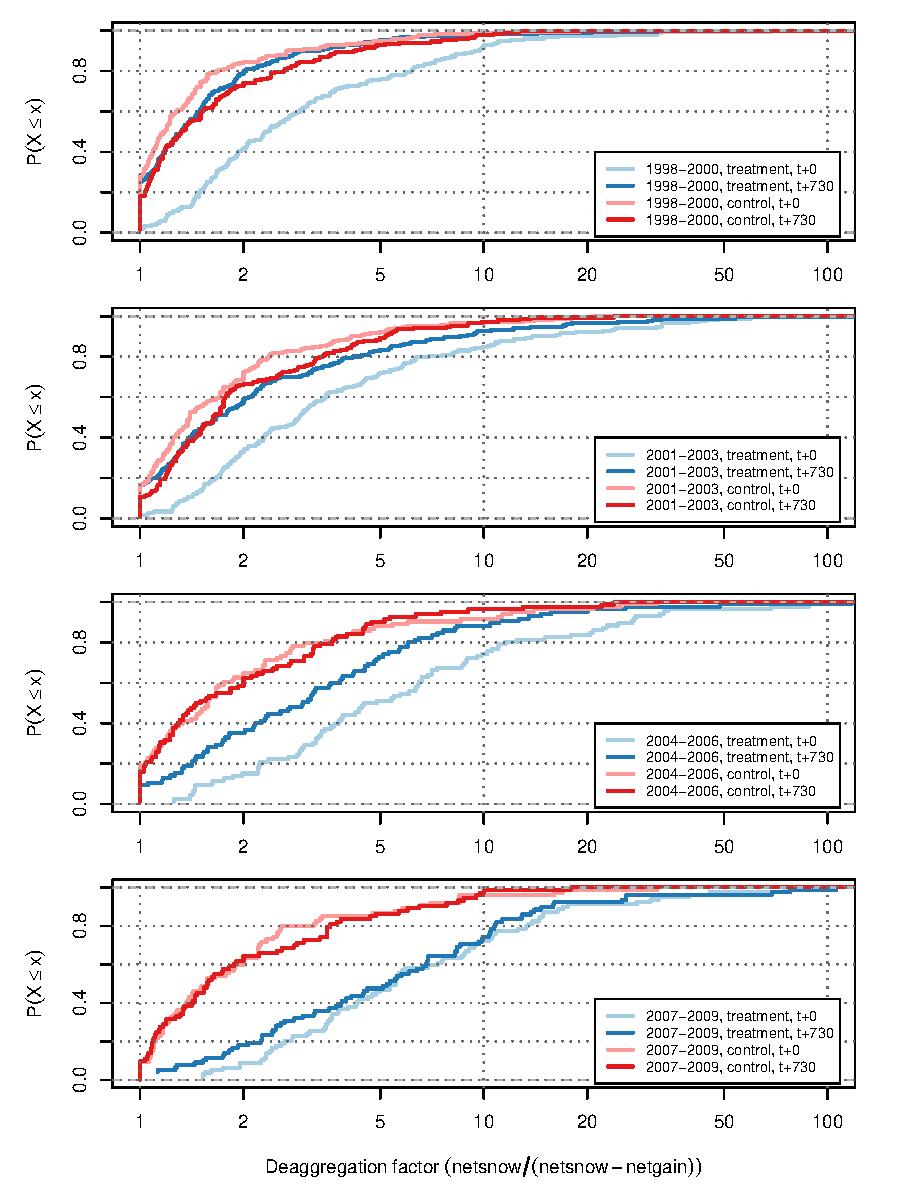
\includegraphics[width=6in]
        {figures/behavior-deagg_factor-vseries-special_tc.pdf}
    \vspace{-2em}\\
    \caption[Simplified deaggregation factor CDFs for four three-year time
    periods over the full data availability period]{Simplified deaggregation
    factor CDFs for four three-year time periods over the full data
    availability period. In all cases, the the data ranges from the first CIDR
    Report of the ending year until the last CIDR Report of the ending year.}
    \label{fig:deagg_factor_cdf_time}
\end{singlespace}
\end{centering}
\end{figure}

In this figure, the light-colored curve represents the deaggregation factor at
the initial measurement time (t+0) and the darker curve of the same color
represents the deaggregation factor at the last measurement time (t+730 days).
As we look at the way the deaggregation factor for treatment and control ASes
changes over time, we can see changes in the apparent response to appearing on
the CIDR Report. The treatment effect (vertical distance between dark and light
lines) was most pronounced in the earliest time period, 1998-2000. The effect
was roughly the same in the 2001-2003 and 2004-2006 periods, with the effect
perhaps even being slightly more pronounced in the later period, especially for
larger DF values. The treatment effect of appearing on the CIDR Report
decreased significantly in the final time period of 2007-2009, with very little
change visible over the various sampling points in the 730 day measurement
window. These results would suggest that the CIDR Report may have been
effective earlier in its life, but has become less effective more recently. The
question of whether the CIDR Report was effective will be discussed more
generally in the following chapter.

Finally, one last view of these data presents a slightly different perspective
by organizing the treatment and control data from the various time periods
together. Figure \ref{fig:deagg_factor_cdf_control} shows the simplified plots
for the control groups for each of the four time periods together in one
figure. While congested and complicated, this suggests visually that the
control groups from each of the periods are in generally good agreement with
each other and do not change greatly with time, except after the first period
where the tendency to deaggregated decreases.

\begin{figure}[H]
\begin{centering}
\begin{singlespace}
    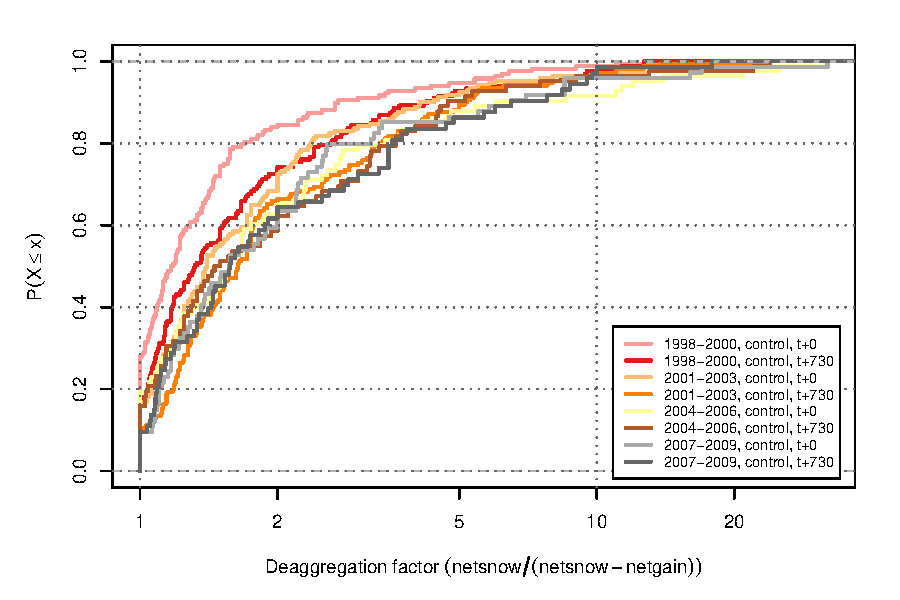
\includegraphics[width=6in]{figures/behavior-deagg_factor-all-special_c.pdf}
    \vspace{-2em}\\
    \caption[Superposition of simplified deaggregation factor CDFs for the
    untreated control ASes]{Superposition of simplified deaggregation factor
    CDFs for the untreated control ASes for the four time periods, showing
    generally similar behavior of untreated ASes throughout time.}
    \label{fig:deagg_factor_cdf_control}
\end{singlespace}
\end{centering}
\end{figure}

Figure \ref{fig:deagg_factor_cdf_treatment} shows the simplified plots for the
treatment groups for each of the four time periods together in one figure.
Unlike the control groups, this figure shows changes across time periods as
well as changes in the apparent response to appearing on the CIDR Report over
time. Each of the time periods is represented by a color, with the initial
(t+0) measurement being in a lighter color and the last (t+730 days)
measurement being in a darker color. First, in terms of the trend between the
four time periods, we can see the trend of increasing deaggregation factor over
time: 80\% of ASes had a DF $\le$ 2 in 1998-2000 after 730 days, and this
steadily decreased across the time periods to just 20\% after 730 days in
2007-2009. We can also observe the change in the treatment effect, though it is
more clearly visible in Figure \ref{fig:deagg_factor_cdf_time}.

\begin{figure}[H]
\begin{centering}
\begin{singlespace}
    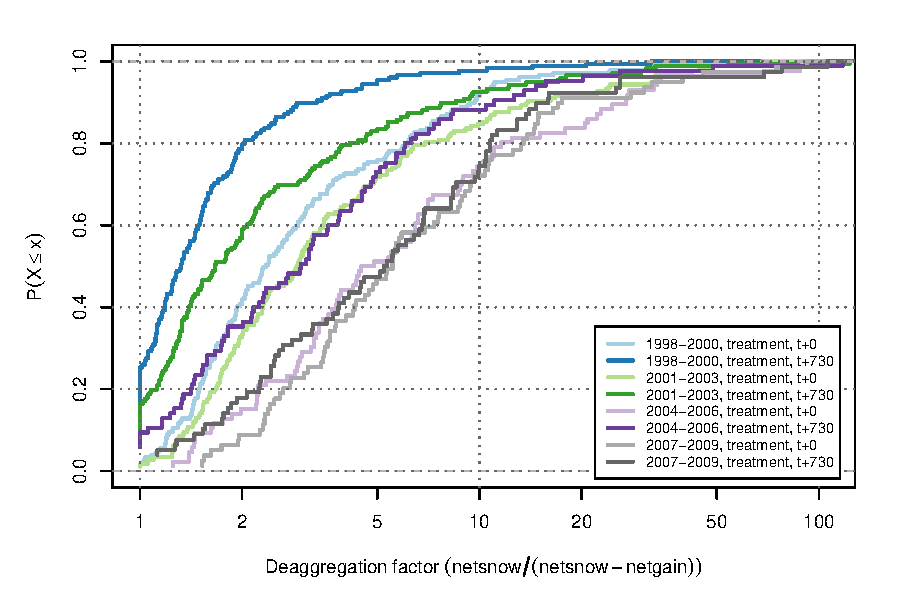
\includegraphics[width=6in]{figures/behavior-deagg_factor-all-special_t.pdf}
    \vspace{-2em}\\
    \caption[Superposition of simplified deaggregation factor CDFs for the
    treated ASes]{Superposition of simplified deaggregation factor CDFs for the
    treated ASes for the four time periods, showing a notable change in
    behavior of ASes appearing on the CIDR Report over time.}
    \label{fig:deagg_factor_cdf_treatment}
\end{singlespace}
\end{centering}
\end{figure}


\subsection{Issues of quasi-experiment validity}
\label{subsec:validity}
One of the challenges of any experiment is achieving validity---being certain
that the conclusions of the experimenter that follow from the results of the
experiment reflect what actually occurred in the experiment
\cite{Babbie:2003uq}. This is particularly critical when attempting to make a
causal inference: that a stimulus really did cause a subsequent effect.
Controlling for sources of invalidity, such as characteristics of the
experimental design or the situation being measured that might confound
results, is relatively easy in laboratory settings, but difficult in real-world
settings, and especially when a quasi-experiment is constructed after the fact
using observational data.  We identify and discuss a number of potential
sources of invalidity, addressing the degree to which each is cause for
questioning the observations made about aggregation behavior following
appearance on the CIDR Report.

\paragraph{Selection bias}

Selection bias refers to the construction of a treatment and control group
whose members are not from the same population, making it impossible to
conclude whether the treatment caused an observed change, as opposed to some
other quality inherent in the treatment or control group members. This is
certainly a potential issue in this analysis of the CIDR Report, as members of
the treatment group, the ASes that appear on the CIDR Report, are by definition
ASes that announce more aggregable prefixes than ASes not on the report (which
are used to form the control group).

It appears that there may be a difference in the population that appears on the
CIDR Report compared to the population of ASes generally, given that many of
the members appearing on the CIDR Report are large ISPs. They may, for
instance, respond differently to the treatment effect of appearing on the CIDR
Report than smaller networks. This may have also affected the deaggregation
factor measure, as large ISPs are more likely to expand their network (and thus
advertise new prefixes) than smaller networks.  This bias was not controlled
for in this study and would be generally difficult to control for because of
the nature of the CIDR Report. Thus, this source of bias cannot be ruled out
through experimental design. However, we may be able to make arguments about
the likely behaviors of large ISPs that in turn allow us to make stronger
arguments about these results.

%TODO expand on this ``stronger arguments'' notion

\paragraph{Regression towards the mean}
Regression towards the mean refers to the selection of a treatment group based
on their having an extreme value for the dependent variable of interest
\cite{Babbie:2003uq}. Over time, members of the group tend towards the
population mean for the dependent variable, appearing to demonstrate a
treatment effect that in reality resulted from tending to the mean. This is
again a potential issue for the CIDR Report, given that the ASes that appear on
the report, and thus are included in the treatment group, are by definition the
ASes that announce the most aggregable prefixes.

In the case of this study, regression to the mean would result in the
appearance of improved aggregation behavior. The control group does not suffer
from such a bias because of its construction by random sampling, and it
suggests that the behavior of untreated ASes remains relatively static over
time.  However, this may not be particularly helpful because the netgain values
of most ASes not on the CIDR report are low, and as in the previous discussion
about selection bias, there is room to question whether the control group is
representative enough because the CIDR Report selects on netgain, the
post-treatment dependent variable.

Both this potential source of bias and the selection bias issue may have been
better controlled with a more tightly specified control group, though it is
unclear what criteria should be used to select a representative control group.
One potential solution is to construct the control group from the group of
ASes that are immediately below the threshold for appearing on the CIDR Report
and so who are theoretically as similar as possible without actually ever
appearing on the CIDR Report. Such a solution would not be as ideal as a
randomized controlled experiment, but would be an improvement for this
quasi-experiment.

% - regression to the mean -- control group shows otherwise, though this is
% perhpas less helpful because the appearance criteria is on netgain -- maybe
% still useful when considering DF?

\paragraph{Failure to measure pre-treatment behavior}

A number of the concerns above about whether the change observed in AS
aggregation behavior following appearance on the CIDR Report could have been
alleviated by measuring pre-treatment behavior---the behavior of ASes that
would eventually appear on the CIDR Report before they appear on the Report. If
a significant change in behavior was observed between pre-treatment and
post-treatment, it would be reasonable to conclude that the CIDR Report did
indeed influence AS behavior.

The failure to measure pre-treatment behavior was an oversight in our
quasi-experimental design. However, because appearance is determined based on
netgain behavior, this may not be as problematic as expected. It is not
possible for an exogenous trend of decreasing netgain to have been occurring
before treatment, for if an AS' netgain were larger than when it first appeared
on the CIDR Report, it would have appeared earlier and thus been subject to
treatment earlier. Thus, we can be reasonably confident that any decreases in
netgain observed were not occurring before treatment occurred, though this
does not rule out previously noted regression or selection effects.

%TODO:
% \paragraph{Other experimental design issues}
% Finally, there are some open questions about this experimental design that,
% while not outright problems, are worth keeping in mind when considering the
% results of this analysis. First, as with any quasi-experiment, it is
% difficult to control all exogenous variables and so another factor could be
% affecting the change in behavior that is not necessarily the CIDR Report. One
% way in which this could be considered is how long would one expect the CIDR
% Report to ``take effect''.
%
%
% - some other behavior at play here? not necessarily the CIDR Report?
%
% - how long should the CIDR Report take to operate?
%
% It is still difficult to tell whether the CIDR Report is having an effect --
% how do we know we are not measuring something else coincident with the CIDR
% Report?  This is difficult to address... Look at large-netsnow with
% low-netgain population??? Future work.
%
% What else could this be measuring that's not improvement in aggregation?
% -ISPs moving prefixes to different ASes
%
% TODO: Other design assumptions and sensitivity to the arbitrary-ness -- 3
% year slices, control with at least 10 prefixes, 30-730 day time windows, etc.

% valdiity notes
% - look at CDF of population elligible to be control
% CIDR Report overall behavior notes
% -> SELECT * FROM get_cumulative_ecr_asns();
% -> SELECT * FROM cumulative_gcr_as_counts;

\subsection{Conclusions}

It is difficult to causally associate appearances on the CIDR Report with
reduction in AS deaggregation behavior with certainty, which would mean that
the CIDR Report did indeed impact AS aggregation behavior without question.
However, there appears to be a discernable correlation between appearing on the
CIDR Report and decreases in the number of aggregable prefixes announced by an
AS.  This effect is more noticeable earlier in the study period, and decreases
as time wears on, with the effect on deaggregation
factor and relative netgain becomes barely distinguishable as of 2007.
% point people at appendix C for further reinforcement

Given this discernable behavior change for ASes on the CIDR Report that is
both different than the control group and that decreases over time,
corroborating qualitative reports of CIDR Report efficacy by network
operators, we are inclined to conclude that the CIDR Report did have some effect
on network operator aggregation behavior, and that this effect decreased over
time. The degree to which this conclusion may be confounded by potential
sources of invalidity limits our inclination to make any stronger claims, though
a qualitative discussion about what this conclusion means and what may have
caused the observed behavior change will proceed in the next chapter.


%////////////////////////////////////////////////////////////////////////////////
%////////////////////////////////////////////////////////////////////////////////
%////////////////////////////////////////////////////////////////////////////////
%IDEA FOR FUTURE ANALYSIS
%
%- Visualization of aggregate behavior and general characteristics (in particular stratification at the top of the CIDR Report)
%    - Definition of metrics used in the analysis
%        - rank on CIDR Report (order by netgain)
%        - absolute/delta netgain
%        - relative/delta netgain (relative to netsnow)
%    - CDFs by AS appearnace
%    - CDFs by rank
%
%    - Summary/general statistics and characteristics of behavior over time (time series?), across and within groups, etc. (p62)
%
%- AS Behavior after appearing on the CIDR Report
%	- Distribution of AS behaviors from T=0, T=+1 month, 3 m, 6m, 1y, 2y, etc.
%		- all appearances on the CIDR Report
%		- no appearance/randomly selected control
%		- appearances that actually had behavior changes observed
%	- slice by date (NOT by rank on CIDR Report), and by netsnow
%
%- Variance in views of data from different peers
%     - for different origin ASes that appear on the CIDR Report
%     - across the entire routing table
